\chapter{Resultados} \label{chap:resultados}
Aquí pondrán las gráficas que obtuvieron en la simulación de matlab para el robot (si las tienen), y las explicarán.

También mostrarán capturas de pantalla de cómo se ve en Gazebo el robot y en RViz, ya sea que funcione o no, para el cambio de trayectoria. Describirán lo que ocurre y por qué (si es que saben).

En la primera gráfica se muestra la evolución de la posición en el espacio cartesiano del efector final del robot a lo largo del tiempo. Las curvas representan las componentes X, Y y Z de dicha posición. Esta gráfica permite analizar cómo se desplaza el efector final en el espacio conforme avanzan los segundos de simulación, y verificar que siga la trayectoria deseada.

La segunda gráfica representa la velocidad lineal del efector final en cada una de las tres direcciones espaciales. Las componentes Vx, Vy y Vz indican con qué rapidez cambia la posición en cada eje. Esta información es útil para analizar si el robot está realizando movimientos suaves o si existen cambios bruscos de velocidad.

En la tercera gráfica se observa la aceleración lineal en los ejes X, Y y Z. Esta métrica refleja cómo cambia la velocidad lineal en el tiempo. Picos en esta gráfica podrían indicar esfuerzos mecánicos altos o comportamientos no deseados que podrían comprometer la estabilidad o el control del robot.


\begin{figure}
	\centering
	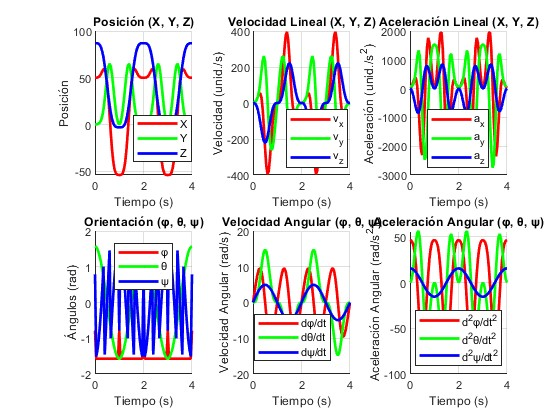
\includegraphics[width=0.5
	\linewidth]{img/cinematicadiferencial}
	\caption{Gráficas Cinemática Diferencial}
	\label{fig:cinematicadiferencial}
\end{figure}

La cuarta gráfica muestra la orientación angular del efector final expresada en términos de los tres ángulos de Euler: phi, theta y psi. Estos ángulos indican cómo rota el efector alrededor de sus propios ejes. Es clave para tareas donde no solo importa la posición, sino también cómo está orientada una herramienta o pinza montada en el extremo.

La quinta gráfica representa la velocidad angular, es decir, qué tan rápido cambian los ángulos de Euler con el tiempo. Se muestran las derivadas respecto al tiempo de phi, theta y psi. Esta gráfica permite verificar si los movimientos rotacionales son suaves y controlados.

Finalmente, la sexta gráfica ilustra la aceleración angular, que es la variación de la velocidad angular. Al igual que con la aceleración lineal, esta información es importante para detectar comportamientos bruscos o posibles problemas de control que afecten la precisión y el rendimiento del robot.
